\documentclass[border = 0.2cm]{standalone}
\usepackage[utf8]{inputenc}

\usepackage{tikz}
\usepackage{amsfonts, amsmath, amssymb}
\usepackage{systeme, mathtools}
\usetikzlibrary{positioning, arrows.meta, quotes}
\usetikzlibrary{shapes,snakes}
\usetikzlibrary{bayesnet}
\tikzset{>=latex}
\tikzstyle{plate caption} = [caption, node distance=0, inner sep=0pt,
below left=5pt and 0pt of #1.south]
\def\outputnames{{$k_a$,$k_{20}$,$k_{23}$,$k_{32}$}}


\begin{document}
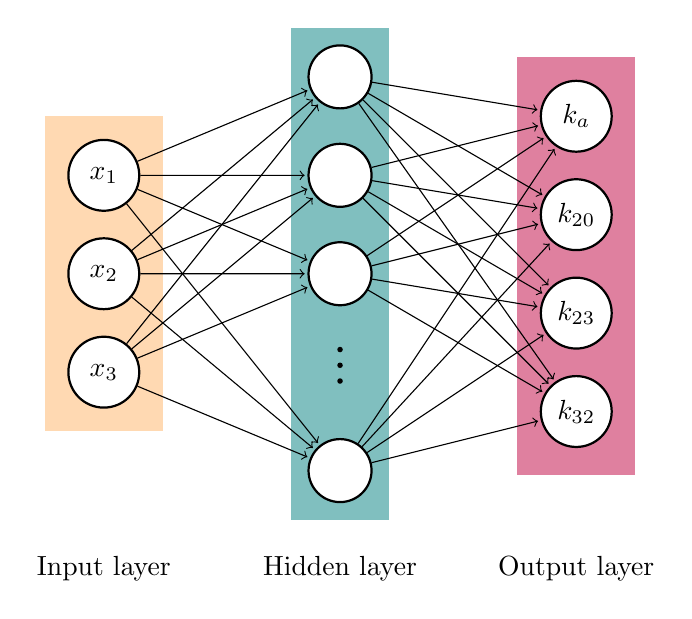
\begin{tikzpicture}
    % Compartment model structure:
    % \node [outer sep=0.15cm] (dose) at (0,2) {$\boldsymbol{\mathrm{D}}$};
    % \node [rectangle, inner sep=0.4cm, thick, dashed, draw] (transit) at (0,0) {Transit};
    % \path [draw,->] (dose) edge (transit);
    % \node [rectangle, inner sep=0.4cm, thick, draw] (central) at (3,0) {Central};
    % \node [outer sep=0.15cm] (k20) at (3,-2) {$k_{20}$};
    % \path [draw,->] (central) edge (k20);
    % \path [draw,->] (transit) edge (central);
    % \node (ka) at (1.5,0.5) {$k_{a}$};
    % \node [rectangle, inner sep=0.4cm, thick, dashed, draw] (periph) at (6,0) {Periph.};
    % \node (k23) at (4.5,0.75) {$k_{23}$};
    % \node (k32) at (4.5,-0.75) {$k_{32}$};
    % \path [draw,->] ([yshift=-2.5mm] periph.west) -- ([yshift=-2.5mm] central.east);
    % \path [draw,->] ([yshift=2.5mm] central.east) -- ([yshift=2.5mm] periph.west);


    % neural network architecture
    % Input layer
    \node (Input layer) at (0, -6.25) {Input layer};
    \node [rectangle, fill=orange!30, minimum width=1.5cm, minimum height=4cm] (Input) at (0, -2.5) {};
    \foreach \i in {1,2,3} {
        \node[circle, minimum size = 9mm, fill=white, thick, draw=black] (Input-\i) at (0,-\i * 1.25) {$x_\i$};
    }
    % Hidden Layer
    \node (x) at (3, -6.25) {Hidden layer};
    \node [rectangle, fill=teal!50, minimum width=1.25cm, minimum height=6.25cm] (Hidden) at (3, -2.5) {};
    \foreach \i in {1,2,3,5} {
        \node[circle, minimum size = 8mm, fill=white, thick, draw=black, yshift=(5-3)*5 mm] (Hidden-\i) at (3,-\i * 1.25 + 0.25) {};
    }
    \foreach \i in {1,...,3} {
        \fill (3, -3.25 * 1.25 + 0.2 * \i) circle (1pt);
    }

    \foreach \i in {1,...,3} {
        \foreach \j in {1,2,3,5} {
            \draw[- {Classical TikZ Rightarrow}, shorten >=1pt] (Input-\i) -- (Hidden-\j);   
        }
    }

    % Output Layer
    \node (x) at (6, -6.25) {Output layer};
    \node [rectangle, fill=purple!50, minimum width=1.5cm, minimum height=5.3cm] (Output) at (6, -2.4) {};
    \node[circle, minimum size = 9mm, fill=white, thick, draw=black, yshift=(5-4)*5 mm] (Output-1) at (6,-1 * 1.25 + 0.25) {$k_a$};
    \node[circle, minimum size = 9mm, fill=white, thick, draw=black, yshift=(5-4)*5 mm] (Output-2) at (6,-2 * 1.25 + 0.25) {$k_{20}$};
    \node[circle, minimum size = 9mm, fill=white, thick, draw=black, yshift=(5-4)*5 mm] (Output-3) at (6,-3 * 1.25 + 0.25) {$k_{23}$};
    \node[circle, minimum size = 9mm, fill=white, thick, draw=black, yshift=(5-4)*5 mm] (Output-4) at (6,-4 * 1.25 + 0.25) {$k_{32}$};

    \foreach \i in {1,2,3,5} {
        \foreach \j in {1,...,4} {
            \draw[- {Classical TikZ Rightarrow}, shorten >=1pt] (Hidden-\i) -- (Output-\j);   
        }
    }
    
\end{tikzpicture}
\end{document}